% Generated by scripts/build.py from content.yaml. Do not edit by hand.
% !TEX program = lualatex
\documentclass[a4paper,10pt]{article}
\usepackage[margin=1.4cm]{geometry}
\usepackage{enumitem,titlesec,xcolor,fontspec,graphicx,fontawesome5,xurl,needspace}
\urlstyle{same}
\usepackage[hidelinks]{hyperref}
\setlength{\parindent}{0pt}\setlength{\parskip}{4pt}
\setlist[itemize]{noitemsep, topsep=0pt, leftmargin=1.5em}
\setlist[enumerate]{topsep=2pt, itemsep=3pt, leftmargin=1.6em}
\renewcommand{\baselinestretch}{1.05}
\definecolor{primary}{HTML}{27438D}\definecolor{muted}{HTML}{5A5A5A}\definecolor{headerbg}{HTML}{C3DFF1}
\setmainfont{Ubuntu}[Path=fonts/, Extension=.ttf, UprightFont=Ubuntu-L, BoldFont=Ubuntu-B, ItalicFont=Ubuntu-LI, BoldItalicFont=Ubuntu-BI]
\hypersetup{colorlinks=true, urlcolor=primary, linkcolor=primary,
  pdftitle={Vipin Singh, CV}, pdfauthor={Vipin Singh}, pdfsubject={Curriculum Vitae},
  pdfkeywords={Holistic model evaluation, Robustness, Time series forecasting, Spatiotemporal modeling, Multimodal deep learning, Uncertainty quantification, Expert-AI collaboration}}
\titleformat{\section}{\needspace{6\baselineskip}\Large\bfseries\color{primary}}{}{0em}{}[\color{primary}\titlerule]
\titlespacing*{\section}{0pt}{7pt}{3pt}
\newcommand{\entry}[4]{\textbf{#1} \hfill \textcolor{muted}{#3}\\\textcolor{muted}{#2\ifx&#4&\else\ \textbf{\textperiodcentered}\ #4\fi}\par}
\begin{document}
\setlength{\fboxsep}{8pt}
\noindent\colorbox{headerbg}{\parbox{\dimexpr\linewidth-2\fboxsep\relax}{%
  \begin{minipage}[c]{0.2\linewidth}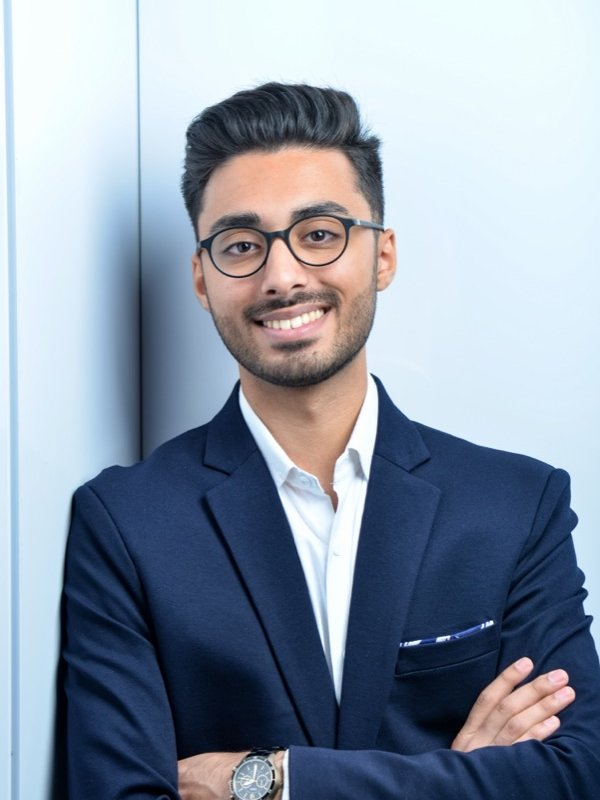
\includegraphics[width=\linewidth]{portrait.jpg}\end{minipage}\hfill
  \begin{minipage}[c]{0.76\linewidth}
    {\LARGE\textbf{Vipin Singh}}\\[3pt]
    \textbf{Data Science Researcher \& Machine Learning Engineer}\\[1pt]
    PhD Candidate in Data Science, Berliner Hochschule für Technik (BHT)\\[5pt]
    \faMapMarker*\ Berlin, Germany\qquad \faEnvelope\ \href{mailto:vipin.singh@bht-berlin.de}{vipin.singh@bht-berlin.de}\\
    \faGlobe\ \href{https://vipin-singh.bio/}{vipin-singh.bio}\qquad \faGithub\ \href{https://github.com/vipin2310}{github.com/vipin2310}\\
    \faLinkedin\ \href{https://www.linkedin.com/in/vipin-singh-131402271}{linkedin.com/in/vipin-singh-131402271}\\
    \faGraduationCap\ \href{https://scholar.google.com/citations?user=9RYzrb4AAAAJ}{Google Scholar}\qquad \faOrcid\ \href{https://orcid.org/0000-0002-4472-8285}{orcid.org/0000-0002-4472-8285}
  \end{minipage}}}

\section*{Profile}
Data science researcher with a background in mathematics and industrial software development. Experienced in building holistic evaluation protocols for machine learning models and managing research projects.

\section*{Experience}
\entry{Research Associate (PhD Candidate), Data Science}{Berliner Hochschule für Technik (BHT)}{Feb 2025 – present}{Berlin, Germany}
\begin{itemize}
  \item Multimodal deep learning models for automatic soil horizon description from profile images and metadata, with BGR.
  \item Spatiotemporal groundwater level prediction at unmonitored locations, with BGR.
  \item Continuation of the RIWWER work packages on time series modeling for urban wastewater management.
\end{itemize}
\entry{Student Research Assistant, Data Science}{Berliner Hochschule für Technik (BHT)}{Dec 2023 – Jan 2025}{Berlin, Germany}
\begin{itemize}
  \item Machine learning models for time series forecasting in urban wastewater management.
  \item Evaluation protocols for predictive performance, model complexity and robustness to data perturbations.
  \item Coordination of the AI work package in the RIWWER research project.
\end{itemize}
\entry{Software Developer, Industrial Image Processing}{NeuroCheck GmbH}{Oct 2018 – Aug 2022}{Stuttgart, Germany}
\begin{itemize}
  \item Image processing and computer vision algorithms for industrial quality inspection systems (C\#, .NET).
  \item Custom image processing modules and plugins for the NeuroCheck software.
  \item Tailored solutions for clients together with engineers and quality assurance specialists.
\end{itemize}
\entry{Intern, System Integration}{Thinking Objects GmbH}{May 2016}{Stuttgart, Germany}


\section*{Education}
\entry{PhD in Data Science (ongoing)}{Berliner Hochschule für Technik (BHT)}{Feb 2025 – present}{}
\begin{itemize}
  \item Supervisor: Prof. Dr. Felix Bießmann
\end{itemize}
\entry{M.Sc. Data Science}{Berliner Hochschule für Technik (BHT)}{Oct 2022 – Jan 2025}{}
\begin{itemize}
  \item Thesis: \textit{Time Series Modeling for Urban Water Management}
  \item Final grade: 1.0 (German scale, 1.0 is best)
\end{itemize}
\entry{B.Sc. Mathematics}{Hochschule für Technik Stuttgart}{Sep 2018 – Aug 2022}{}
\begin{itemize}
  \item Thesis: \textit{Development of a Deflectometry-based Inspection System for Reflective Surfaces}
  \item Final grade: 1.3 (German scale, 1.0 is best)
\end{itemize}

\section*{Research Projects}
\textbf{Groundwater level prediction at unmonitored locations} \textcolor{muted}{(2025–present, with BGR)}\par\smallskip
\textbf{SoilNet, AI-assisted soil horizon description} \textcolor{muted}{(2025–present, with BGR)}\\
\href{https://soilnet.demo.calgo-lab.de/}{Live demo} \textbf{\textperiodcentered} \href{https://github.com/calgo-lab/BGR}{Code} \textbf{\textperiodcentered} \href{https://www.bgr.bund.de/}{BGR}\par\smallskip
\textbf{RIWWER, resilient forecasting for urban sewer systems} \textcolor{muted}{(2023–present, with University of Duisburg-Essen and partners)}\\
\href{https://riwwer.demo.calgo-lab.de/}{Live demo} \textbf{\textperiodcentered} \href{https://github.com/calgo-lab/resilient-timeseries-evaluation}{Code} \textbf{\textperiodcentered} \href{https://www.riwwer.fraunhofer.de/}{Project}\par\smallskip

\section*{Publications}
\begin{enumerate}
  \item \textbf{Vipin Singh}, Joey Prüssing, Teodor Chiaburu, Einar Eberhardt, Sina Hesse, Stefan Broda, Frank Haußer, Felix Bießmann. \textit{SoilNet App: AI-Assisted Expert-level Annotations of Soil Horizons}. IJCAI-ECAI 2026, Demo Track, 2026. \href{https://doi.org/10.24963/ijcai.2026/993}{\nolinkurl{doi:10.24963/ijcai.2026/993}}
  \item \textbf{Vipin Singh}, Tianheng Ling, Peter Ghaly, Felix Grimmeisen, Gregor Schiele, Felix Bießmann. \textit{A Resilient Solution for Sewer Overflow Monitoring Across Cloud and Edge}. IJCAI-ECAI 2026, Demo Track, 2026. \href{https://doi.org/10.24963/ijcai.2026/994}{\nolinkurl{doi:10.24963/ijcai.2026/994}}
  \item \textbf{Vipin Singh}$^*$, Teodor Chiaburu$^*$, Einar Eberhardt, Stefan Broda, Joey Prüssing, Frank Haußer$^\dagger$, Felix Bießmann$^\dagger$. \textit{SoilNet: A multimodal multitask model for hierarchical classification of soil horizons}. Geoderma, 2026. \href{https://doi.org/10.1016/j.geoderma.2026.117684}{\nolinkurl{doi:10.1016/j.geoderma.2026.117684}} {\small\textcolor{muted}{($^*$equal contribution; $^\dagger$equal supervision)}}
  \item Teodor Chiaburu, \textbf{Vipin Singh}, Frank Haußer$^\dagger$, Felix Bießmann$^\dagger$. \textit{Uncertainty-Guided Expert-AI Collaboration for Efficient Soil Horizon Annotation}. ECAI 2025 Workshop, 2025. \href{https://arxiv.org/abs/2509.24873}{\nolinkurl{arXiv:2509.24873}} {\small\textcolor{muted}{($^\dagger$equal supervision)}}
  \item Tianheng Ling$^*$, \textbf{Vipin Singh}$^*$, Chao Qian, Felix Bießmann, Gregor Schiele. \textit{Automated Energy-Aware Time-Series Model Deployment on Embedded FPGAs for Resilient Combined Sewer Overflow Management}. IEEE ISC2 2025, 2025. \href{https://doi.org/10.1109/ISC266238.2025.11293267}{\nolinkurl{doi:10.1109/ISC266238.2025.11293267}} {\small\textcolor{muted}{($^*$equal contribution)}}
  \item \textbf{Vipin Singh}, Tianheng Ling, Teodor Chiaburu, Felix Bießmann. \textit{Evaluating Time Series Models for Urban Wastewater Management: Predictive Performance, Model Complexity and Resilience}. SpliTech 2025, 2025. \href{https://doi.org/10.23919/SpliTech65624.2025.11091801}{\nolinkurl{doi:10.23919/SpliTech65624.2025.11091801}}
  \item \textbf{Vipin Singh}, Tianheng Ling, Teodor Chiaburu, Felix Bießmann. \textit{Data-driven Modeling of Combined Sewer Systems for Urban Sustainability: An Empirical Evaluation}. KI 2024 Workshop, 2024. \href{https://arxiv.org/abs/2408.11619}{\nolinkurl{arXiv:2408.11619}}
\end{enumerate}


\section*{Skills and Languages}
\textbf{Programming:} Python, C\#, Java\\
\textbf{Machine learning:} PyTorch, scikit-learn, OpenCV, pandas, NumPy\\
\textbf{Tools:} Git, Linux, Docker, Kubernetes\\
\textbf{Languages:} German (native), English (fluent), Hindi (proficient)


\vfill{\footnotesize\textcolor{muted}{Last updated 2026-10-07. Current version: \href{https://vipin-singh.bio/}{vipin-singh.bio}}}
\end{document}
